% Options for packages loaded elsewhere
\PassOptionsToPackage{unicode}{hyperref}
\PassOptionsToPackage{hyphens}{url}
%
\documentclass[
  english,
  ,doc,floatsintext]{apa6}
\usepackage{lmodern}
\usepackage{amsmath}
\usepackage{ifxetex,ifluatex}
\ifnum 0\ifxetex 1\fi\ifluatex 1\fi=0 % if pdftex
  \usepackage[T1]{fontenc}
  \usepackage[utf8]{inputenc}
  \usepackage{textcomp} % provide euro and other symbols
  \usepackage{amssymb}
\else % if luatex or xetex
  \usepackage{unicode-math}
  \defaultfontfeatures{Scale=MatchLowercase}
  \defaultfontfeatures[\rmfamily]{Ligatures=TeX,Scale=1}
\fi
% Use upquote if available, for straight quotes in verbatim environments
\IfFileExists{upquote.sty}{\usepackage{upquote}}{}
\IfFileExists{microtype.sty}{% use microtype if available
  \usepackage[]{microtype}
  \UseMicrotypeSet[protrusion]{basicmath} % disable protrusion for tt fonts
}{}
\makeatletter
\@ifundefined{KOMAClassName}{% if non-KOMA class
  \IfFileExists{parskip.sty}{%
    \usepackage{parskip}
  }{% else
    \setlength{\parindent}{0pt}
    \setlength{\parskip}{6pt plus 2pt minus 1pt}}
}{% if KOMA class
  \KOMAoptions{parskip=half}}
\makeatother
\usepackage{xcolor}
\IfFileExists{xurl.sty}{\usepackage{xurl}}{} % add URL line breaks if available
\IfFileExists{bookmark.sty}{\usepackage{bookmark}}{\usepackage{hyperref}}
\hypersetup{
  pdftitle={Supplementary Materials: Effects of human-animal interactions on affect and cognition},
  pdfauthor={Elise R. Thayer1 \& Jeffrey R. Stevens1},
  pdflang={en-EN},
  hidelinks,
  pdfcreator={LaTeX via pandoc}}
\urlstyle{same} % disable monospaced font for URLs
\usepackage{graphicx}
\makeatletter
\def\maxwidth{\ifdim\Gin@nat@width>\linewidth\linewidth\else\Gin@nat@width\fi}
\def\maxheight{\ifdim\Gin@nat@height>\textheight\textheight\else\Gin@nat@height\fi}
\makeatother
% Scale images if necessary, so that they will not overflow the page
% margins by default, and it is still possible to overwrite the defaults
% using explicit options in \includegraphics[width, height, ...]{}
\setkeys{Gin}{width=\maxwidth,height=\maxheight,keepaspectratio}
% Set default figure placement to htbp
\makeatletter
\def\fps@figure{htbp}
\makeatother
\setlength{\emergencystretch}{3em} % prevent overfull lines
\providecommand{\tightlist}{%
  \setlength{\itemsep}{0pt}\setlength{\parskip}{0pt}}
\setcounter{secnumdepth}{-\maxdimen} % remove section numbering
% Make \paragraph and \subparagraph free-standing
\ifx\paragraph\undefined\else
  \let\oldparagraph\paragraph
  \renewcommand{\paragraph}[1]{\oldparagraph{#1}\mbox{}}
\fi
\ifx\subparagraph\undefined\else
  \let\oldsubparagraph\subparagraph
  \renewcommand{\subparagraph}[1]{\oldsubparagraph{#1}\mbox{}}
\fi
% Manuscript styling
\usepackage{upgreek}
\captionsetup{font=singlespacing,justification=justified}

% Table formatting
\usepackage{longtable}
\usepackage{lscape}
% \usepackage[counterclockwise]{rotating}   % Landscape page setup for large tables
\usepackage{multirow}		% Table styling
\usepackage{tabularx}		% Control Column width
\usepackage[flushleft]{threeparttable}	% Allows for three part tables with a specified notes section
\usepackage{threeparttablex}            % Lets threeparttable work with longtable

% Create new environments so endfloat can handle them
% \newenvironment{ltable}
%   {\begin{landscape}\begin{center}\begin{threeparttable}}
%   {\end{threeparttable}\end{center}\end{landscape}}
\newenvironment{lltable}{\begin{landscape}\begin{center}\begin{ThreePartTable}}{\end{ThreePartTable}\end{center}\end{landscape}}

% Enables adjusting longtable caption width to table width
% Solution found at http://golatex.de/longtable-mit-caption-so-breit-wie-die-tabelle-t15767.html
\makeatletter
\newcommand\LastLTentrywidth{1em}
\newlength\longtablewidth
\setlength{\longtablewidth}{1in}
\newcommand{\getlongtablewidth}{\begingroup \ifcsname LT@\roman{LT@tables}\endcsname \global\longtablewidth=0pt \renewcommand{\LT@entry}[2]{\global\advance\longtablewidth by ##2\relax\gdef\LastLTentrywidth{##2}}\@nameuse{LT@\roman{LT@tables}} \fi \endgroup}

% \setlength{\parindent}{0.5in}
% \setlength{\parskip}{0pt plus 0pt minus 0pt}

% \usepackage{etoolbox}
\makeatletter
\patchcmd{\HyOrg@maketitle}
  {\section{\normalfont\normalsize\abstractname}}
  {\section*{\normalfont\normalsize\abstractname}}
  {}{\typeout{Failed to patch abstract.}}
\patchcmd{\HyOrg@maketitle}
  {\section{\protect\normalfont{\@title}}}
  {\section*{\protect\normalfont{\@title}}}
  {}{\typeout{Failed to patch title.}}
\makeatother
\shorttitle{Supplementary Materials}
\usepackage{csquotes}
\usepackage[justification=Centering,position=top]{subfig}
\ifxetex
  % Load polyglossia as late as possible: uses bidi with RTL langages (e.g. Hebrew, Arabic)
  \usepackage{polyglossia}
  \setmainlanguage[]{english}
\else
  \usepackage[shorthands=off,main=english]{babel}
\fi
\ifluatex
  \usepackage{selnolig}  % disable illegal ligatures
\fi

\title{Supplementary Materials: Effects of human-animal interactions on affect and cognition}
\author{Elise R. Thayer\textsuperscript{1} \& Jeffrey R. Stevens\textsuperscript{1}}
\date{}


\affiliation{\vspace{0.5cm}\textsuperscript{1} University of Nebraska-Lincoln}

\begin{document}
\maketitle

\renewcommand{\thetable}{S\arabic{table}}
\setcounter{table}{0}
\renewcommand{\thefigure}{S\arabic{figure}}
\setcounter{figure}{0}

\renewcommand{\arraystretch}{1.35}

\clearpage

\begin{table}

\caption{\label{tab:dems}Demographics}
\centering
\fontsize{9}{11}\selectfont
\begin{tabular}[t]{lll}
\toprule
\multicolumn{1}{c}{} & \multicolumn{1}{c}{Experiment 1} & \multicolumn{1}{c}{Experiment 2} \\
\cmidrule(l{3pt}r{3pt}){2-2} \cmidrule(l{3pt}r{3pt}){3-3}
Measure & $N$ (\%) & $N$ (\%)\\
\midrule
Age (M(SD)) & 19.0 (1.4) & 20.0 (1.8)\\
\addlinespace[0.3em]
\multicolumn{3}{l}{\textbf{Gender}}\\
\hspace{1em}Female & 60 (82.2) & 66 (79.5)\\
\hspace{1em}Male & 13 (17.8) & 17 (20.5)\\
\hspace{1em}Other & 0 (0) & 0 (0)\\
\addlinespace[0.3em]
\multicolumn{3}{l}{\textbf{Race/Ethnicity}}\\
\hspace{1em}Asian & 6 (8.2) & 9 (10.8)\\
\hspace{1em}Black & 5 (6.8) & 5 (6)\\
\hspace{1em}Native American & 0 (0) & 3 (3.6)\\
\hspace{1em}Pacific Islander & 0 (0) & 0 (0)\\
\hspace{1em}White/Caucasian & 58 (79.5) & 58 (69.9)\\
\hspace{1em}Other & 4 (5.5) & 8 (9.6)\\
\addlinespace[0.3em]
\multicolumn{3}{l}{\textbf{Family Income}}\\
\hspace{1em}< \$25000 & 3 (4.1) & 5 (6)\\
\hspace{1em}\$25000-\$50000 & 6 (8.2) & 12 (14.5)\\
\hspace{1em}\$50000-\$75000 & 9 (12.3) & 15 (18.1)\\
\hspace{1em}\$75000-\$100000 & 17 (23.3) & 13 (15.7)\\
\hspace{1em}> \$100000 & 32 (43.8) & 31 (37.3)\\
\hspace{1em}Preferred not to answer & 6 (8.2) & 7 (8.4)\\
\bottomrule
\multicolumn{3}{l}{\textsuperscript{} Note:}\\
\end{tabular}
\end{table}

\begin{table}

\caption{\label{tab:unnamed-chunk-2}Words used in Deese-Roedinger-McDermott long-term memory test.}
\centering
\begin{tabular}[t]{ll}
\toprule
Presentation words & Recall words\\
\midrule
kid & kid*\\
adult & toy*\\
adolescent & immature*\\
toy & beaker*\\
parent & physics*\\
\addlinespace
baby & test tube*\\
dependent & child\\
immature & chemistry\\
brat & blouse\\
juvenile & table\\
\addlinespace
beaker & victory\\
element & cardboard\\
lab & \\
physics & \\
formula & \\
\addlinespace
molecule & \\
flask & \\
test tube & \\
scientist & \\
electron & \\
\bottomrule
\multicolumn{2}{l}{\textsuperscript{*} Denotes recall words that were}\\
\multicolumn{2}{l}{present in presentation phase.}\\
\multicolumn{2}{l}{\textsuperscript{} Note:}\\
\end{tabular}
\end{table}

\clearpage
\newpage



\begin{figure}
\subfloat[\label{fig:tasks-fig-1}]{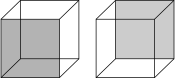
\includegraphics[width=0.45\linewidth]{/mnt/data/jstevens/OneDrive/active_sync/projects/haicognition2021/figures/illustration_necker_cube} }\hspace{5mm}\subfloat[\label{fig:tasks-fig-2}]{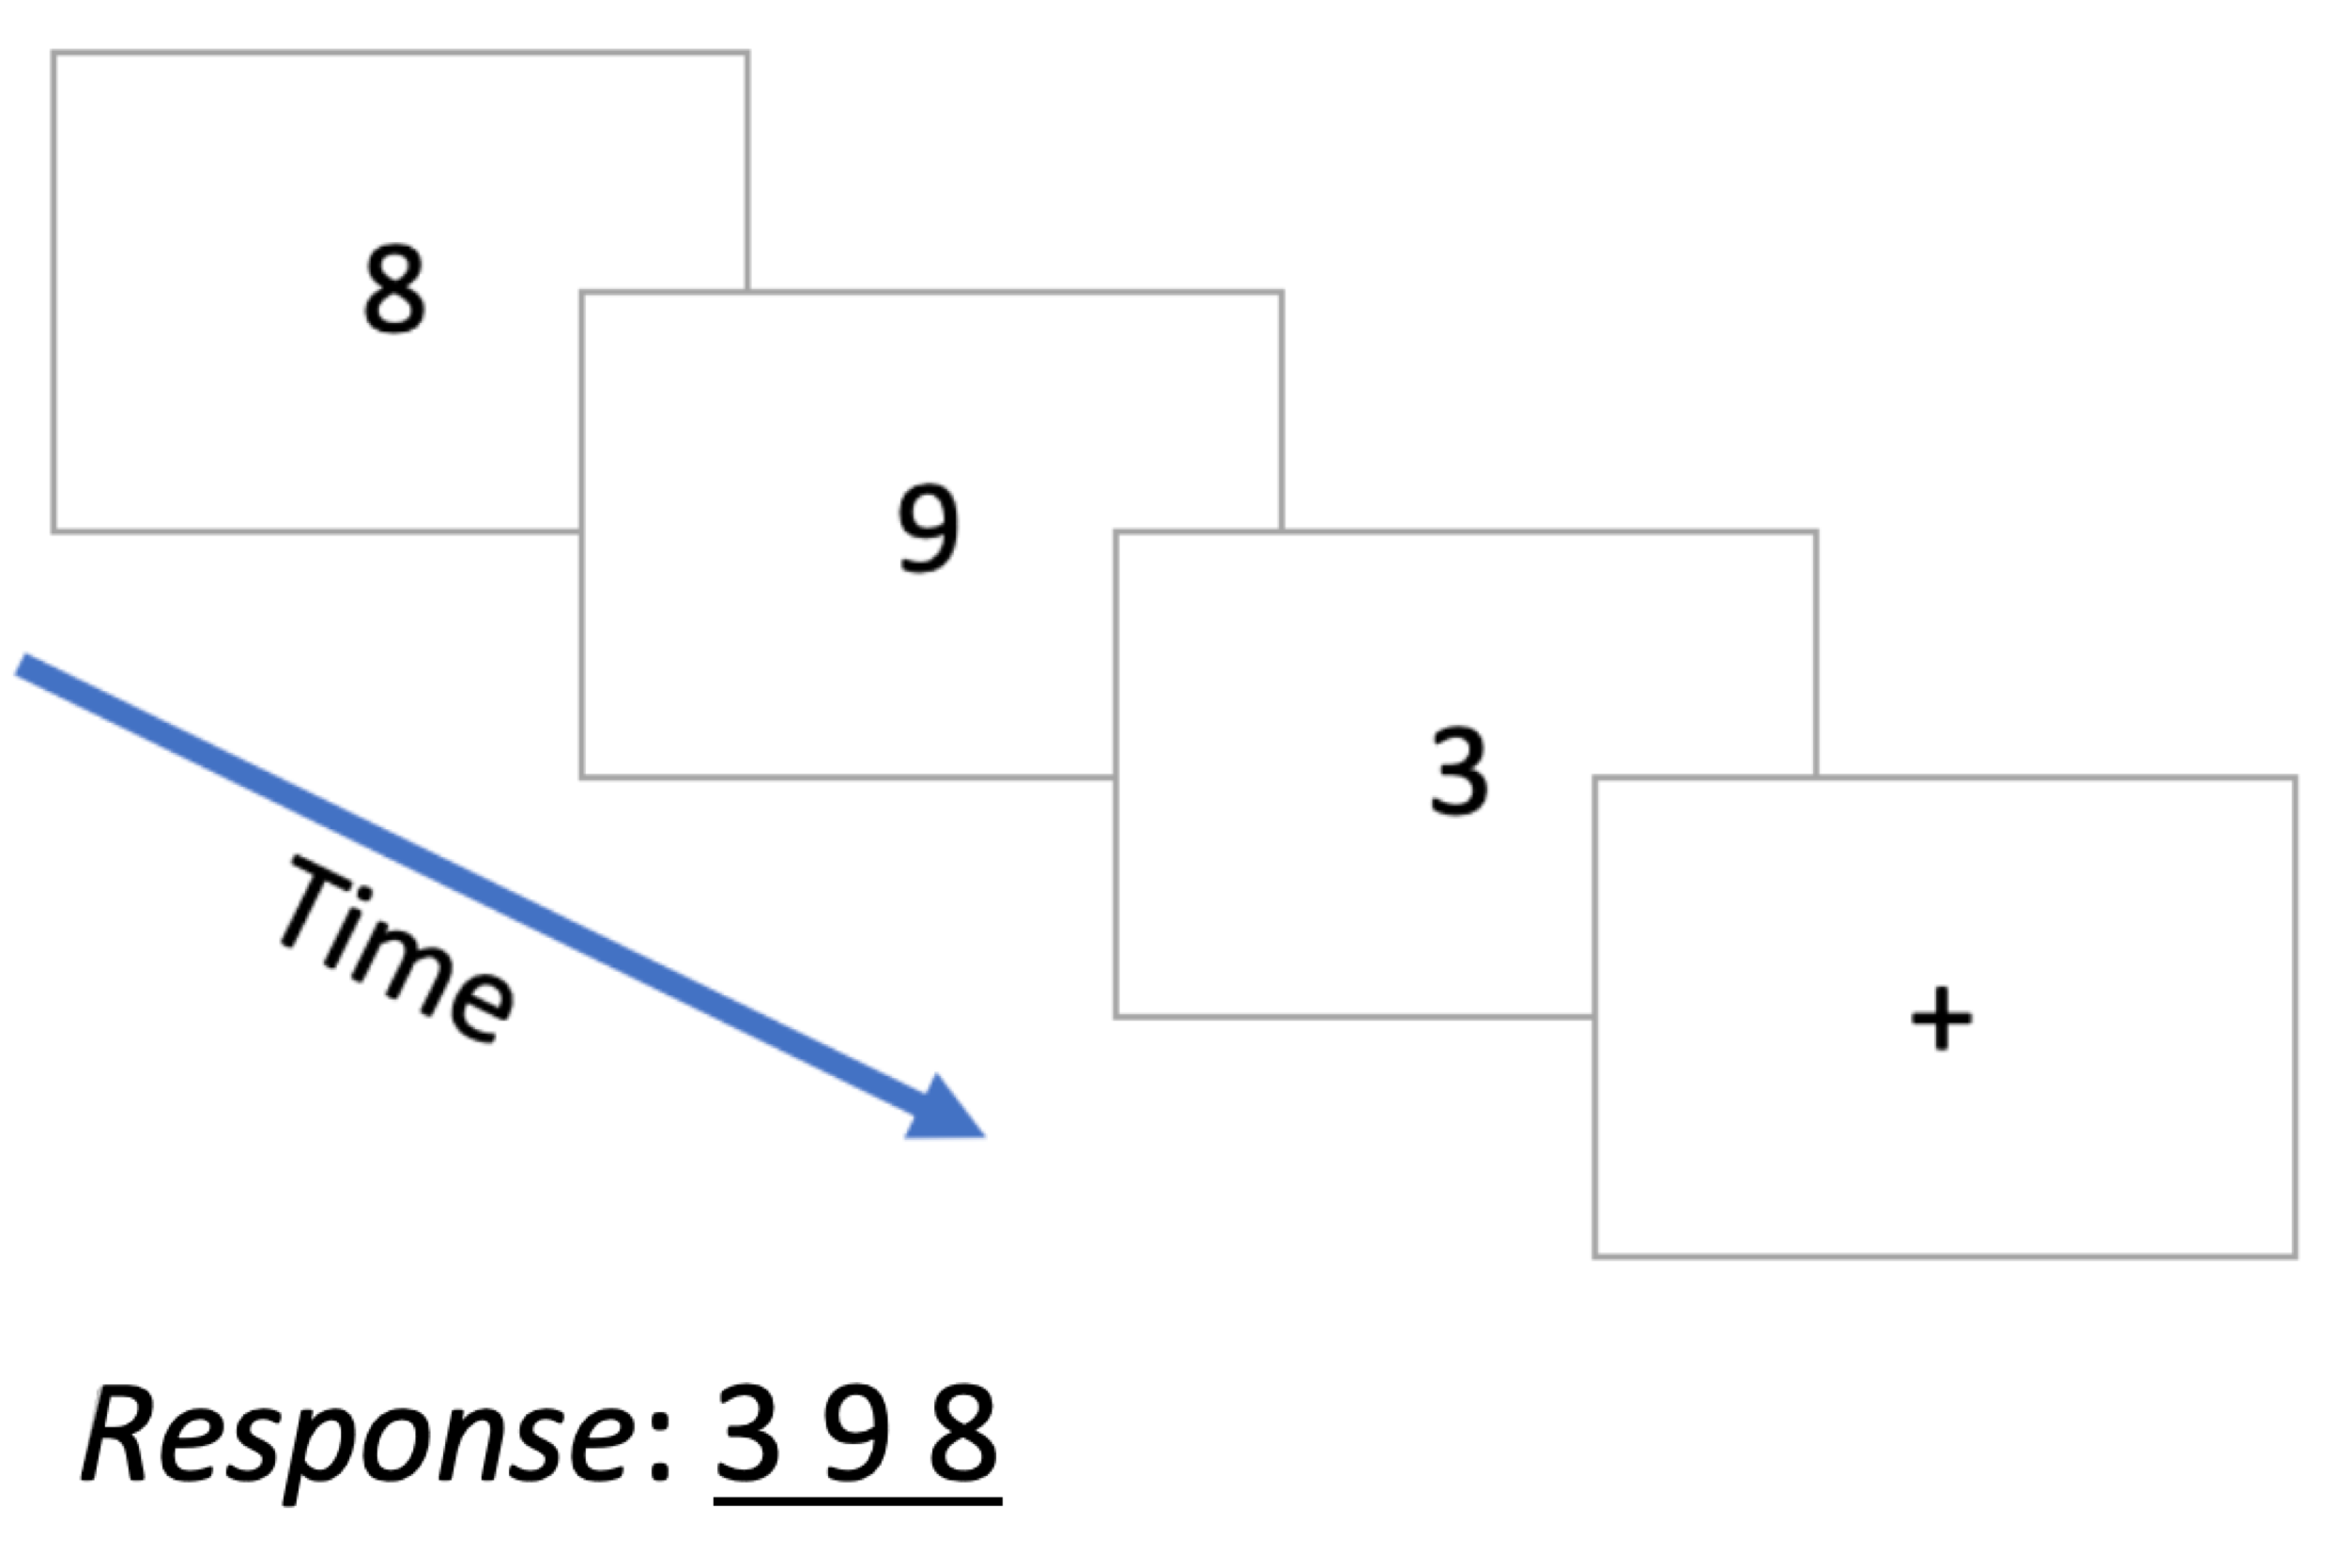
\includegraphics[width=0.45\linewidth]{/mnt/data/jstevens/OneDrive/active_sync/projects/haicognition2021/figures/illustration_backwards_digit_span} }\newline\subfloat[\label{fig:tasks-fig-3}]{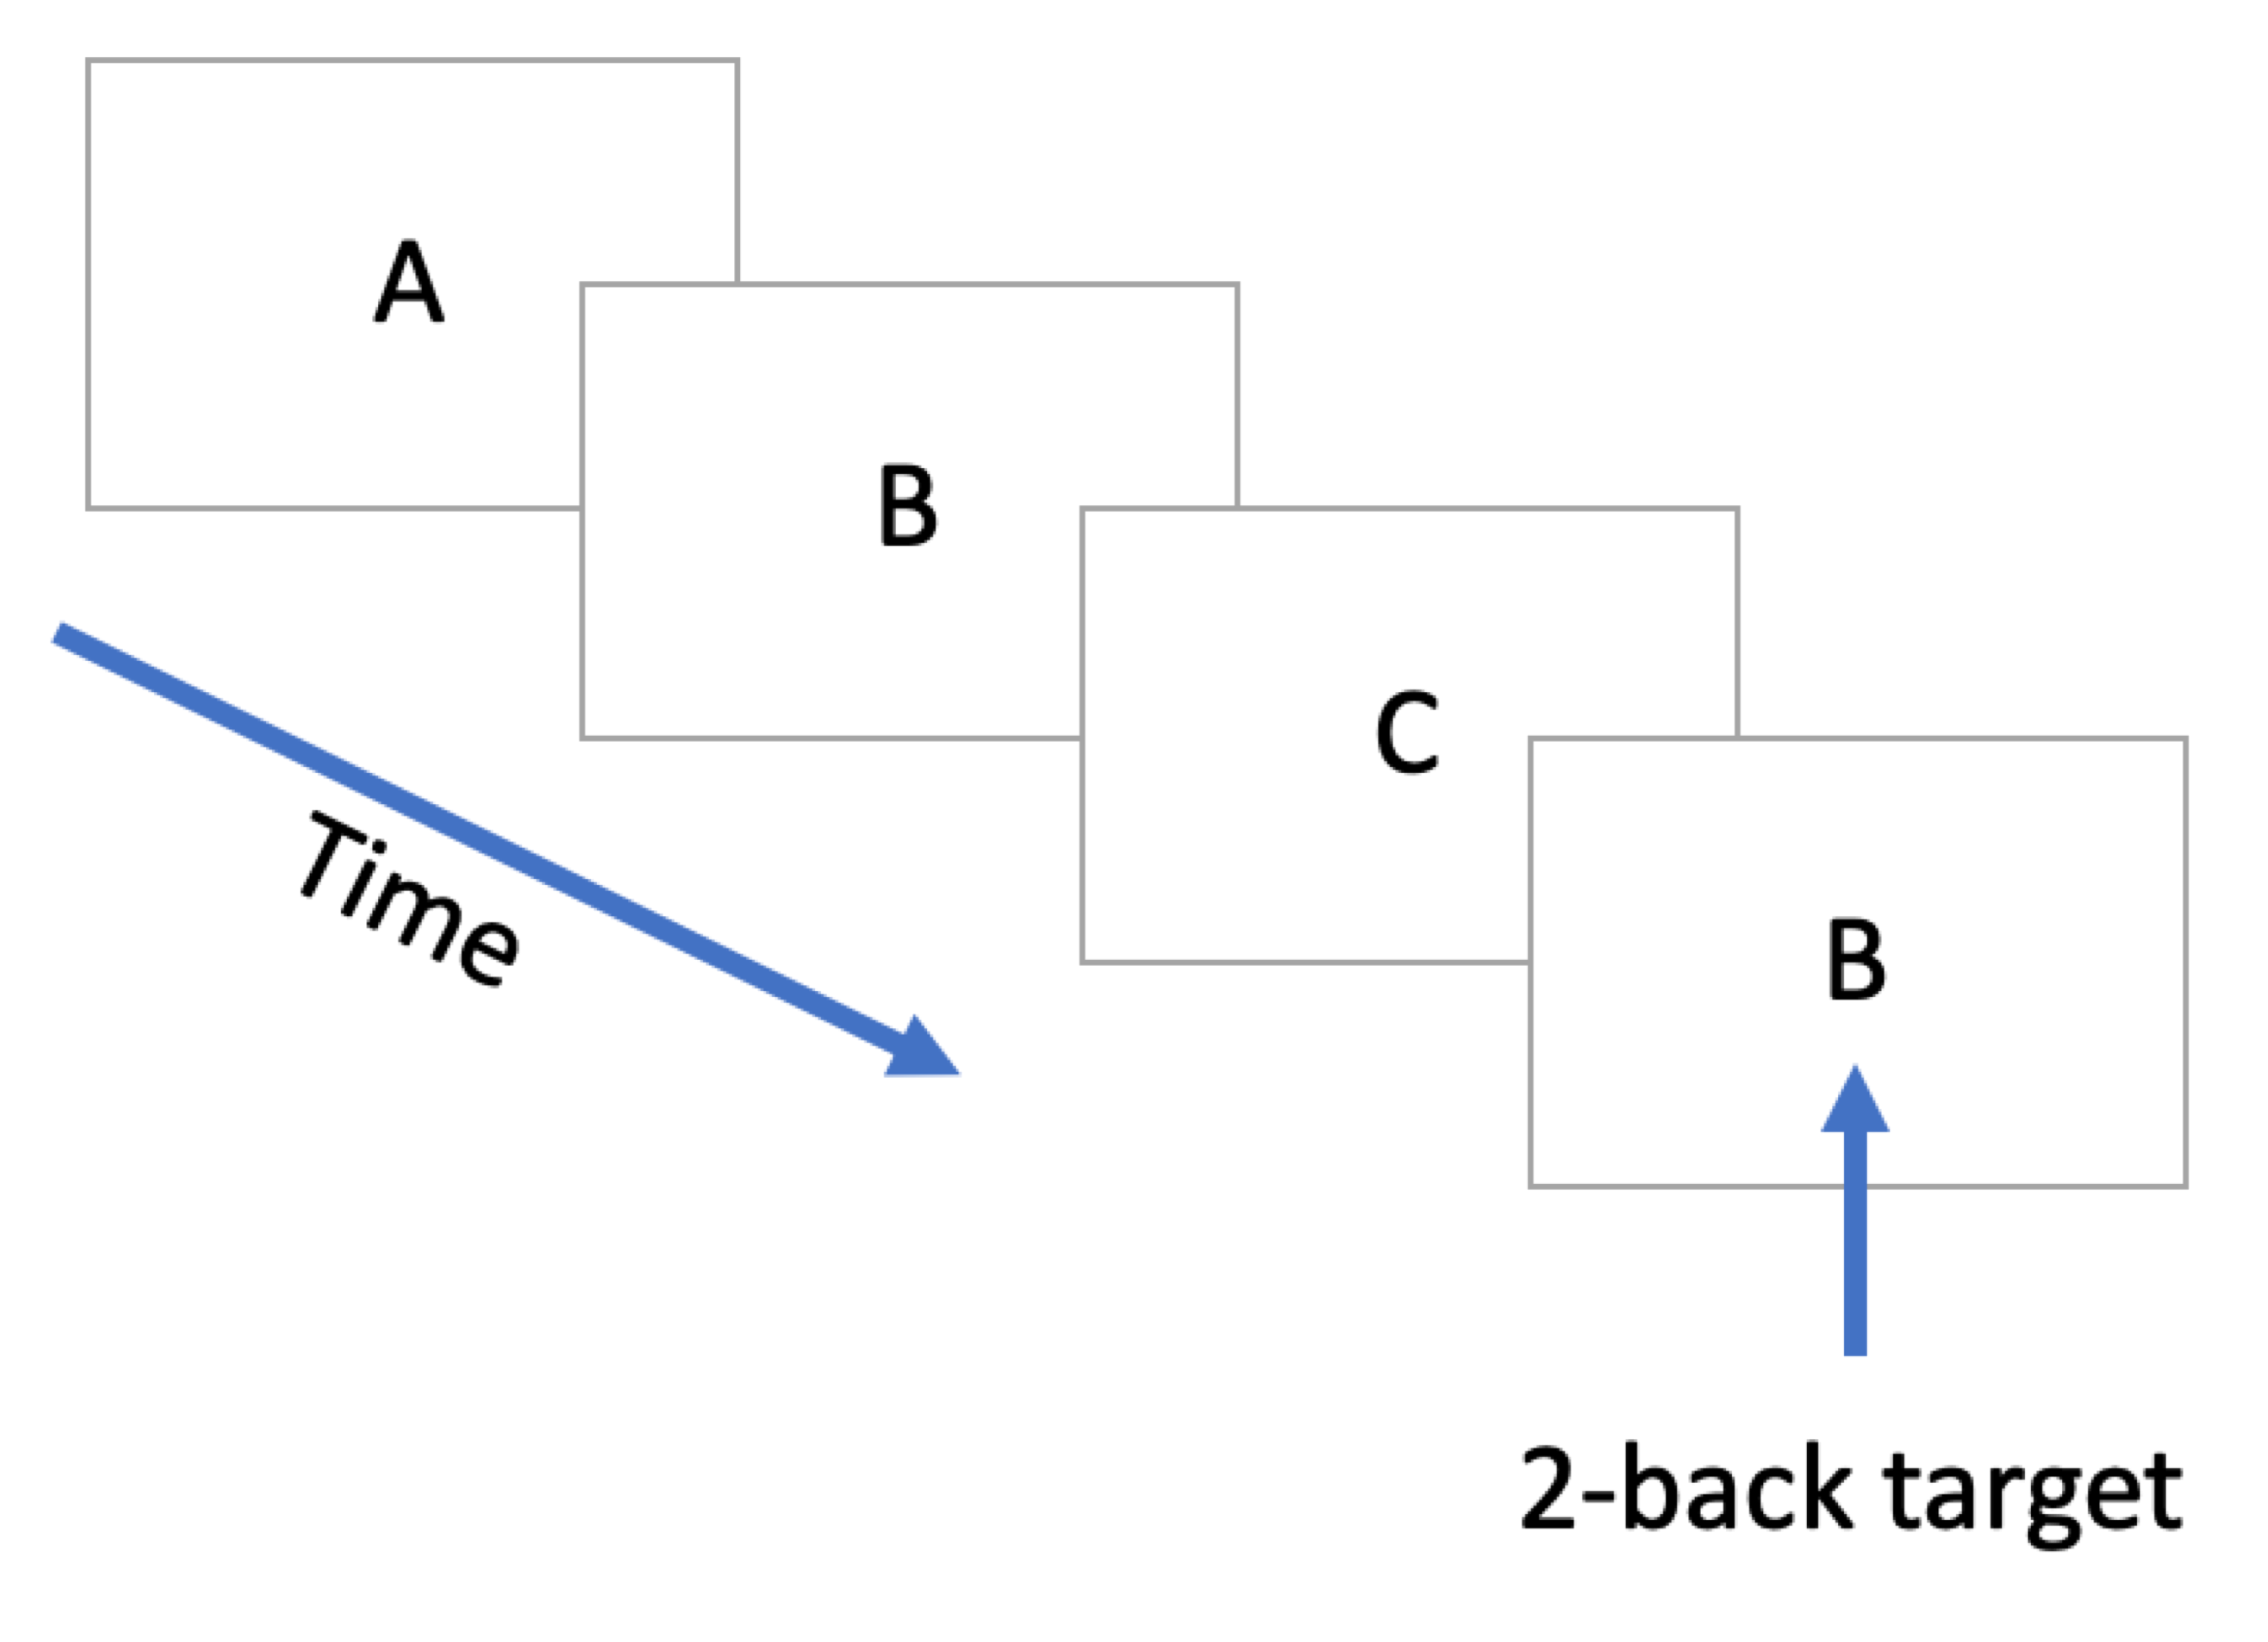
\includegraphics[width=0.45\linewidth]{/mnt/data/jstevens/OneDrive/active_sync/projects/haicognition2021/figures/illustration_n-back} }\caption{Cognitive tasks: (a) Necker Cube Pattern Control Test, (b) backwards digit span test, and (c) n-back task.}\label{fig:tasks-fig}
\end{figure}



\begin{figure}
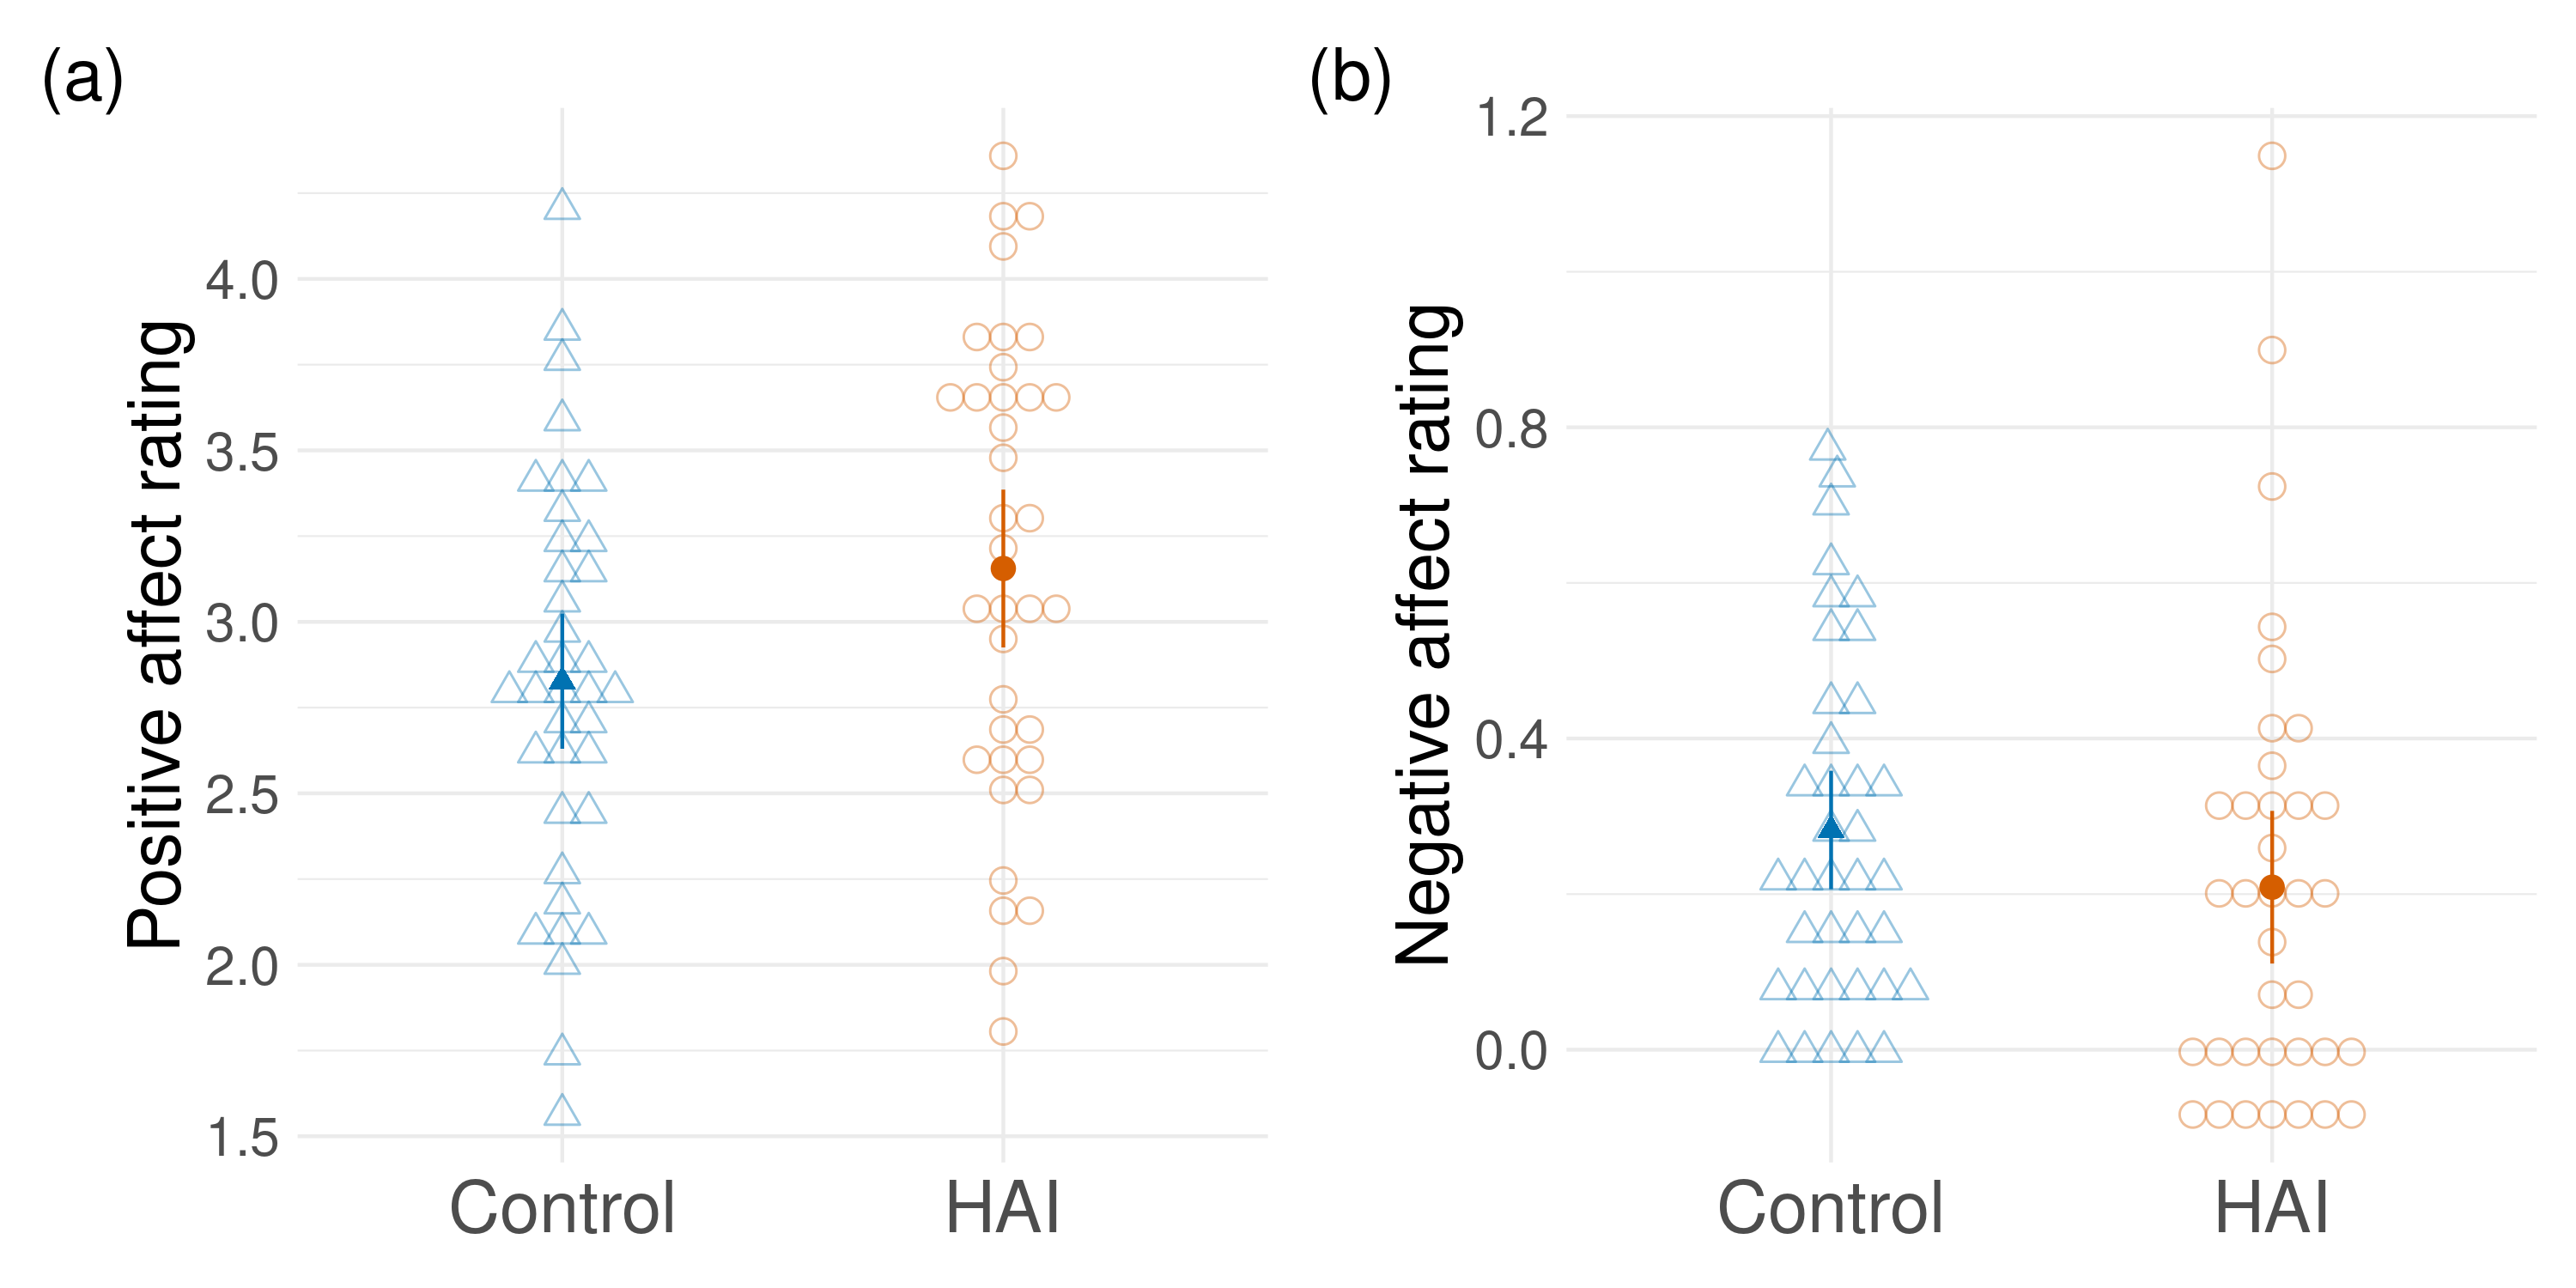
\includegraphics[width=1\linewidth]{/mnt/data/jstevens/OneDrive/active_sync/projects/haicognition2021/figures/affect_1} \caption{Post-condition predicted affect scores (controlling for pre-condition scores) for control and HAI (human-animal interaction) groups in Experiment 1. Scores show (a) positive PANAS ratings and (b) negative PANAS ratings. Negative affect scores are log-transformed. Open triangles (blue) represent individual control participant scores, open circles (orange) represent individual HAI participant scores, closed triangles and circles represent condition group means (with lines connecting condition means), error bars represent 95\% confidence intervals.}\label{fig:affect1}
\end{figure}



\begin{figure}
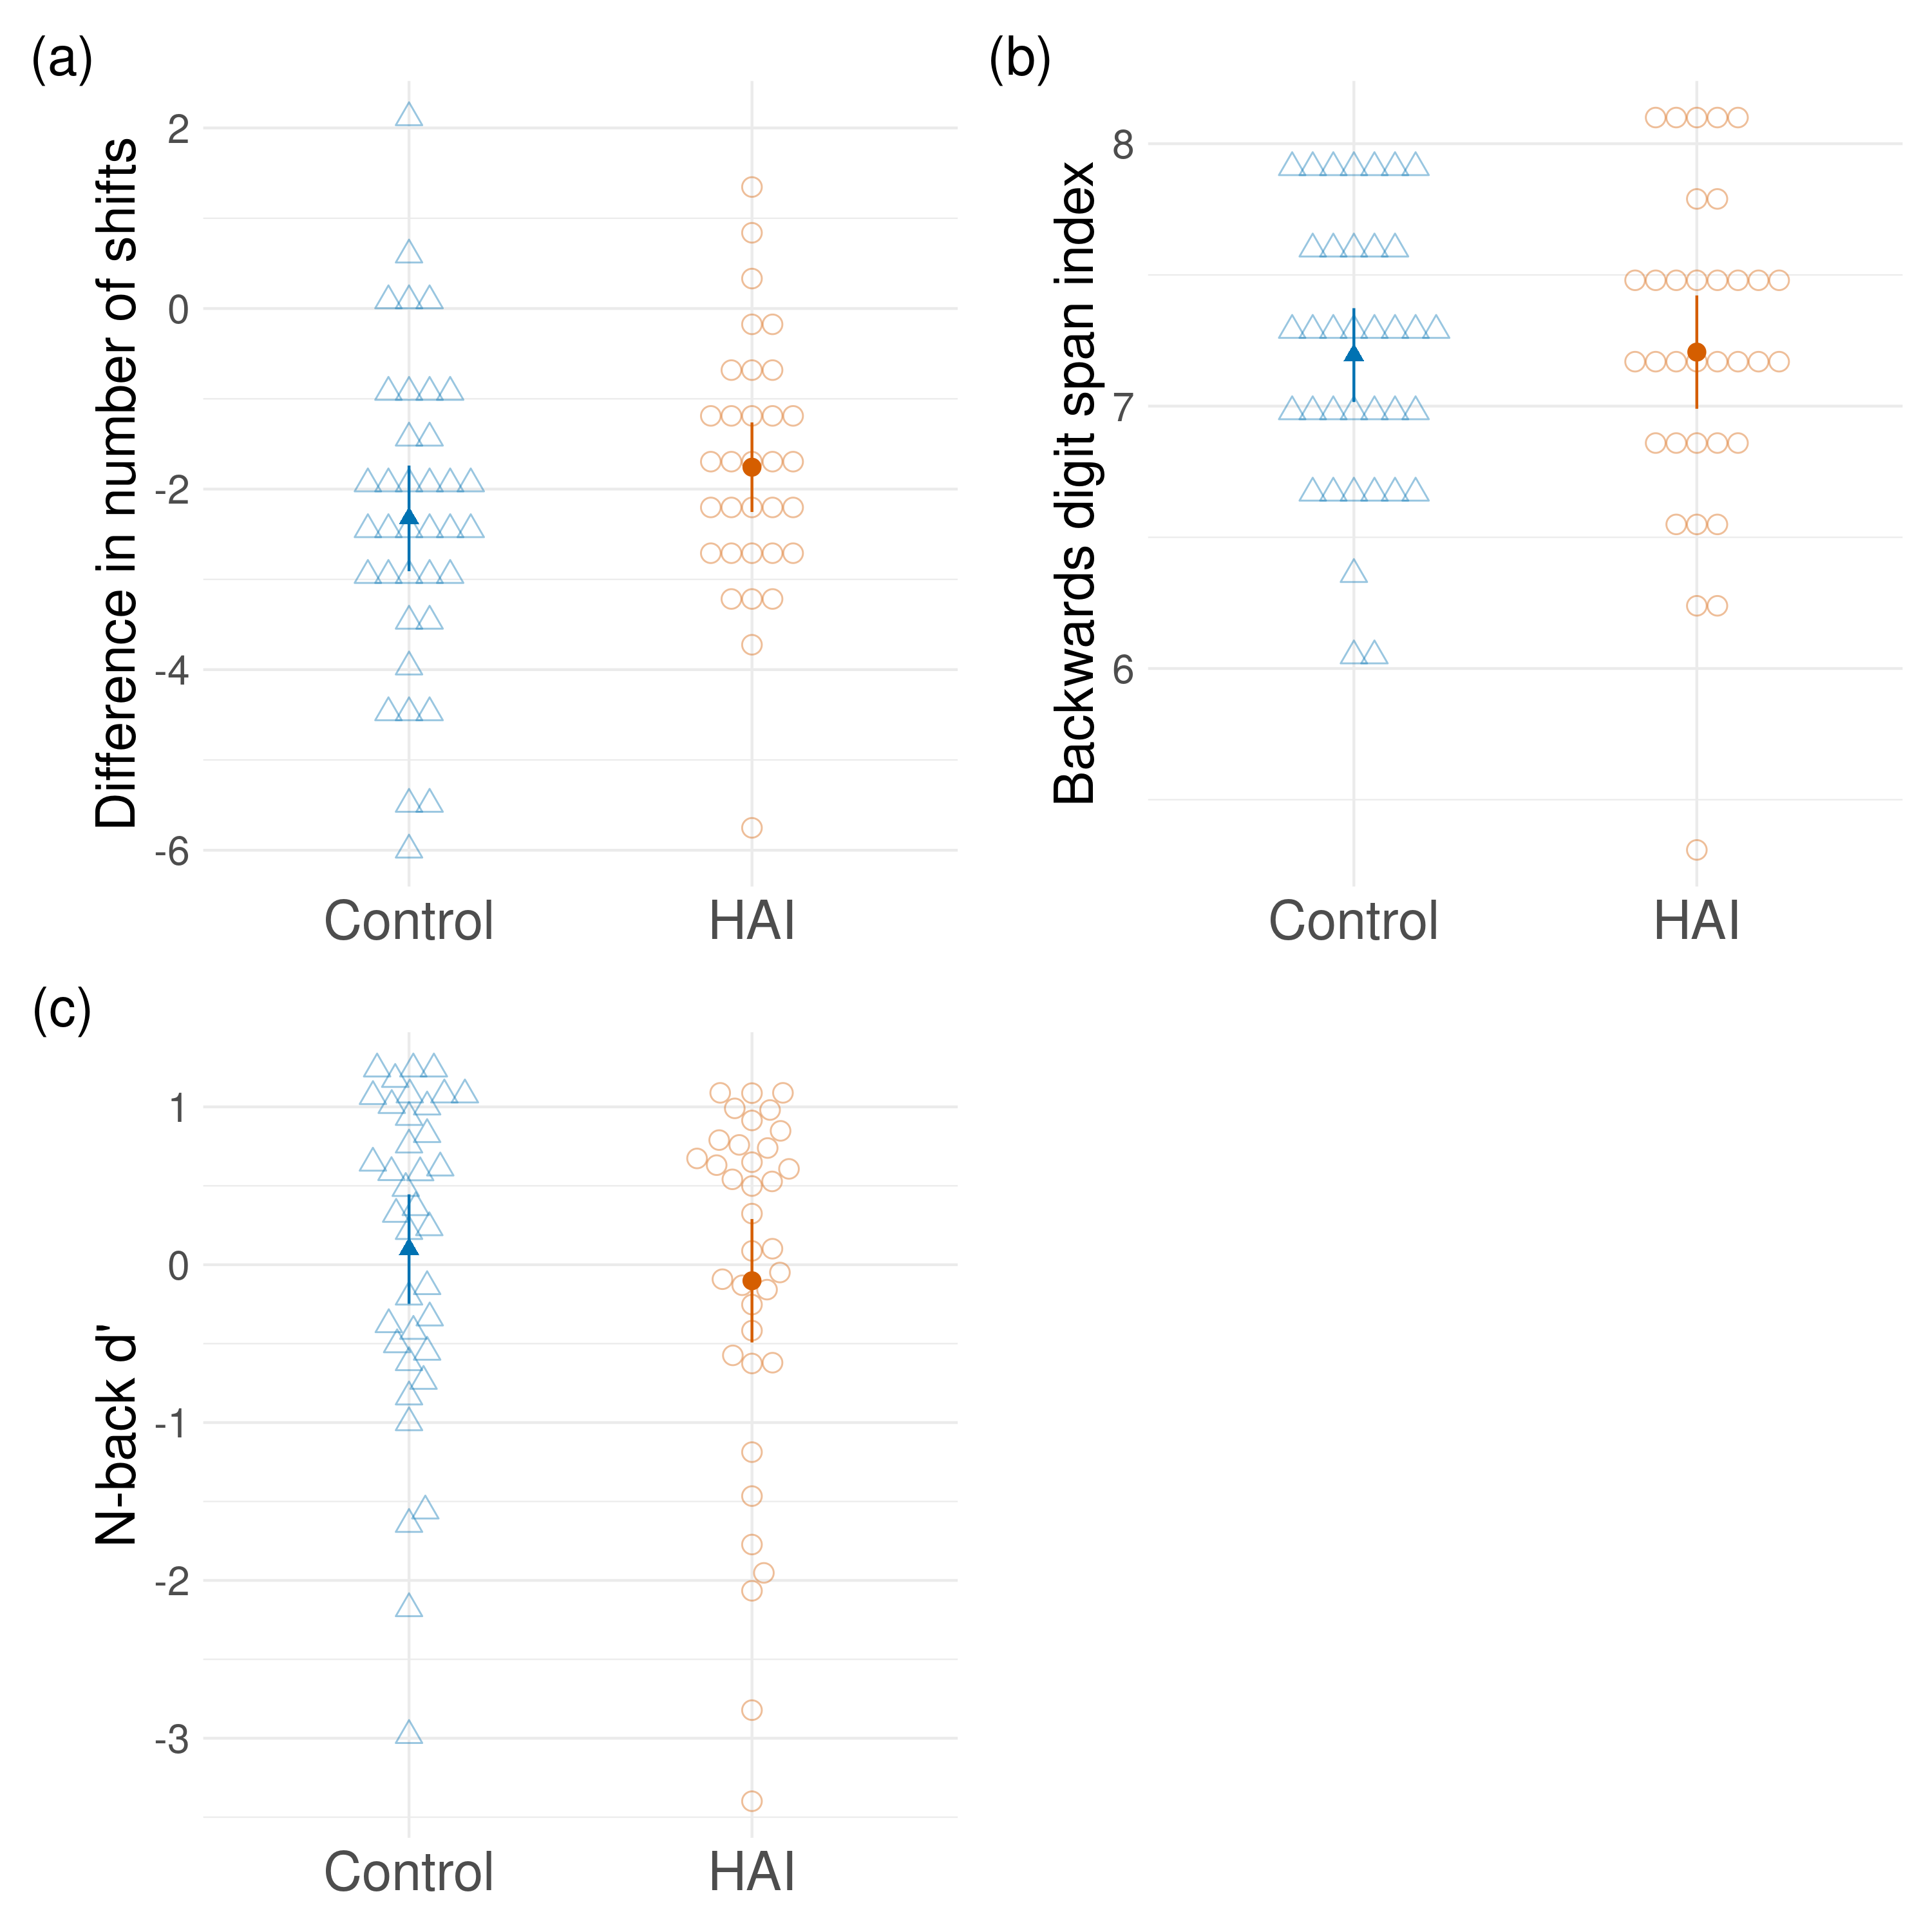
\includegraphics[width=1\linewidth]{/mnt/data/jstevens/OneDrive/active_sync/projects/haicognition2021/figures/cognitive_1} \caption{Post-condition predicted cognitive scores (controlling for pre-condition scores) for HAI (human-animal interaction) and control groups in Experiment 1. Scores show (a) the difference in number of attentional shifts between the two Necker cube trials, (b) the index for the backwards digit span task, and (c) \(d'\) for the n-back task. Open triangles (blue) represent individual control participant scores, open circles (orange) represent individual HAI participant scores, closed triangles and circles represent condition group means (with lines connecting condition means), error bars represent 95\% confidence intervals.}\label{fig:cognitive1}
\end{figure}



\begin{figure}

{\centering 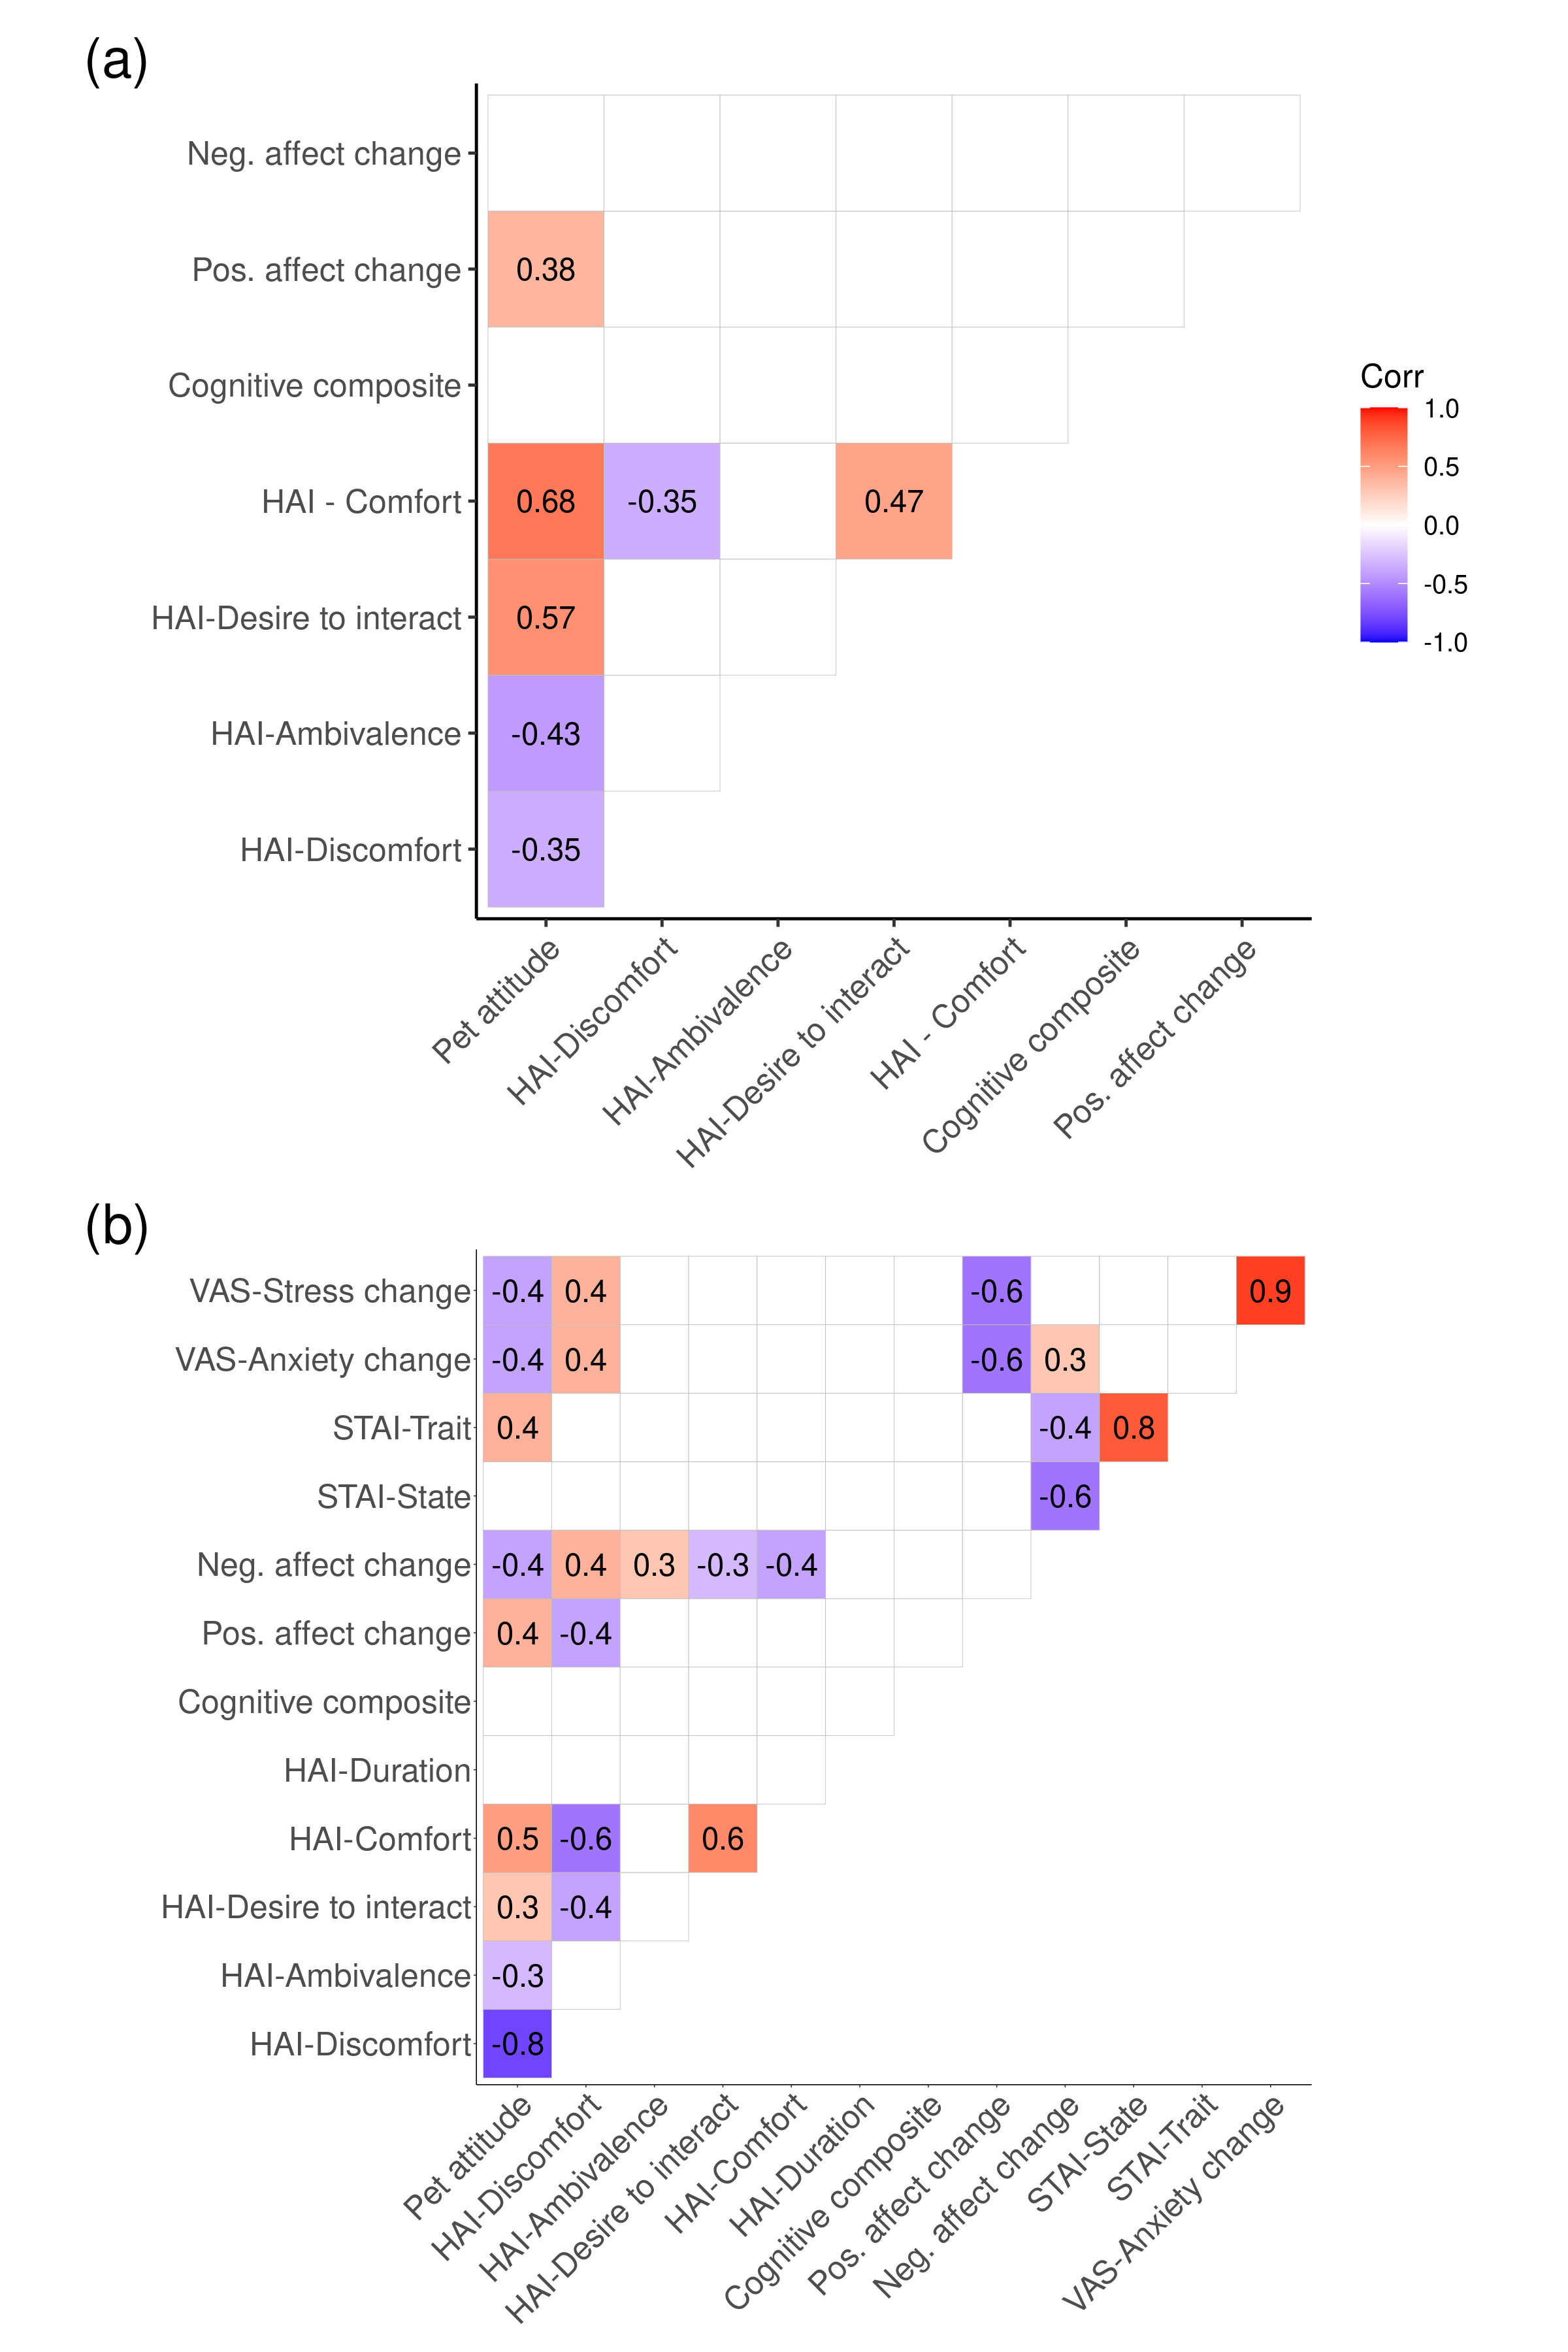
\includegraphics[width=0.8\linewidth]{/mnt/data/jstevens/OneDrive/active_sync/projects/haicognition2021/figures/correlation_plots} 

}

\caption{Animal experience correlation matrices for Experiments 1 (a) and 2 (b). Values in cells are correlation coefficients for correlations with p \textless{} 0.05.}\label{fig:hai-corr-plots}
\end{figure}



\begin{figure}
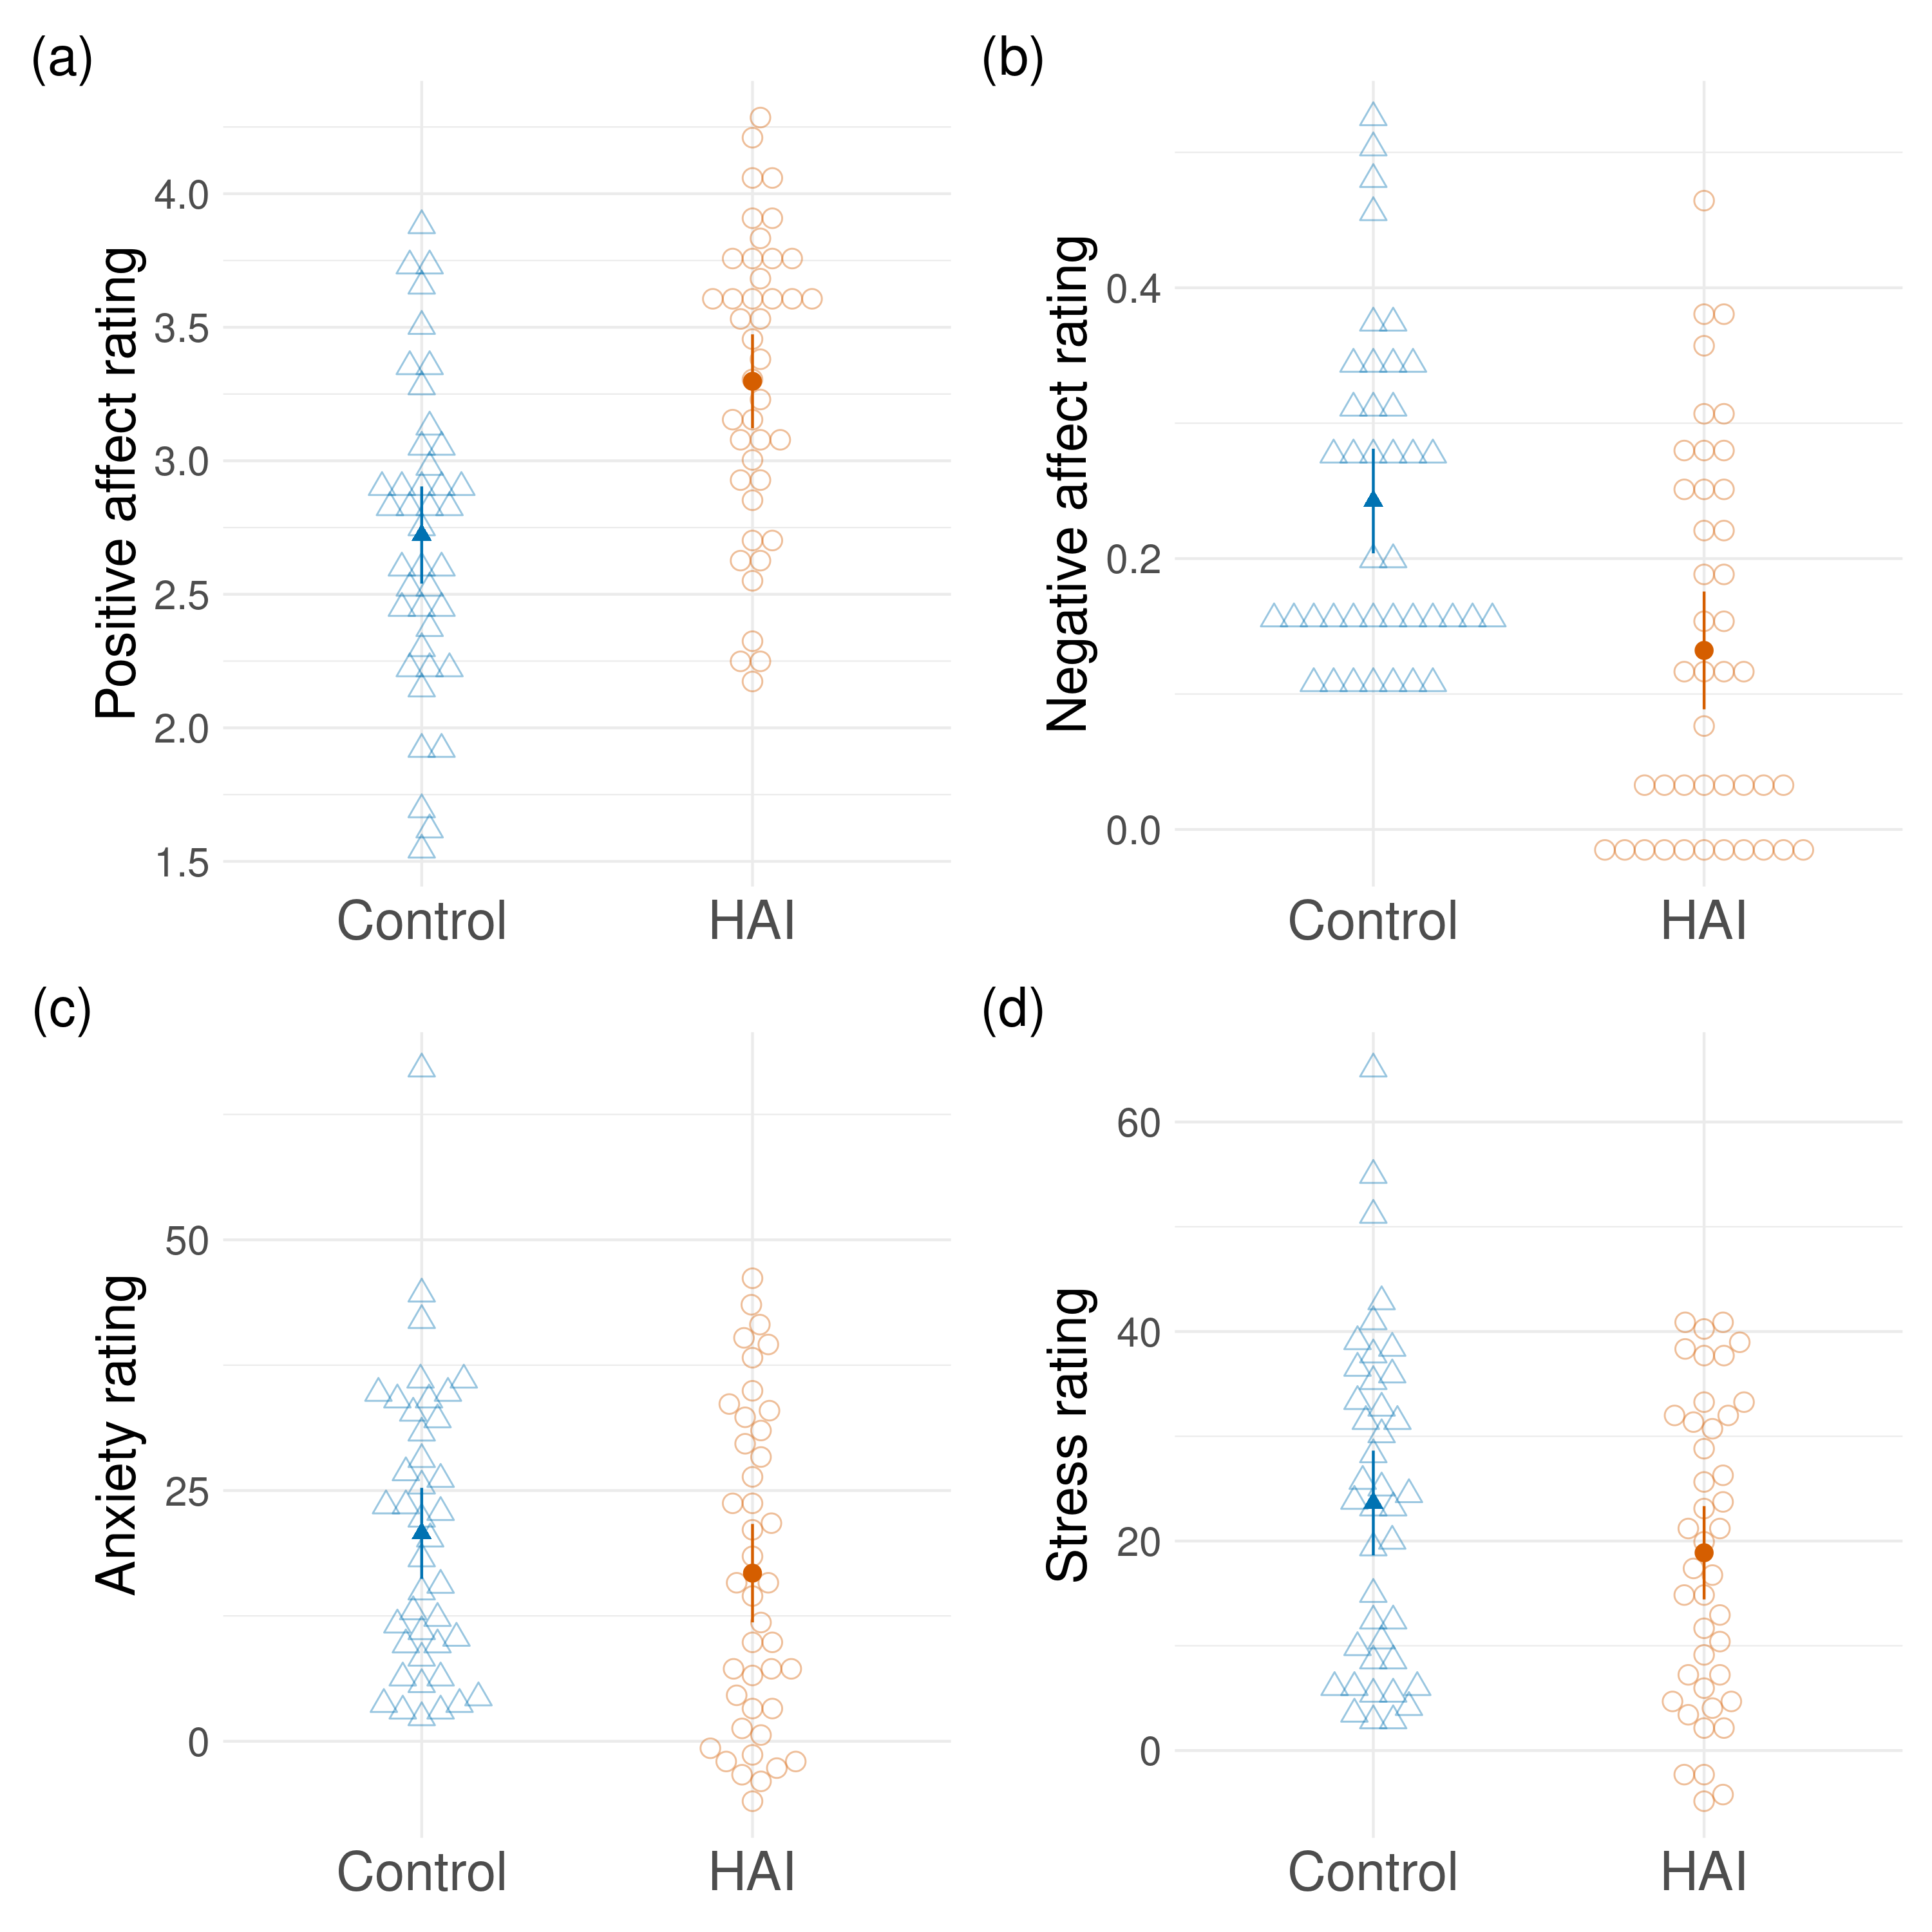
\includegraphics[width=1\linewidth]{/mnt/data/jstevens/OneDrive/active_sync/projects/haicognition2021/figures/affect_2} \caption{Post-condition predicted affect scores (controlling for pre-condition scores) for control and HAI (human-animal interaction) groups in Experiment 2. Scores show (a) positive PANAS ratings, (b) negative PANAS ratings, (c) anxiety ratings, and (d) stress ratings. Negative affect scores are log-transformed. Open triangles (blue) represent individual control participant scores, open circles (orange) represent individual HAI participant scores, closed triangles and circles represent condition group means (with lines connecting condition means), error bars represent 95\% confidence intervals.}\label{fig:affect2}
\end{figure}



\begin{figure}
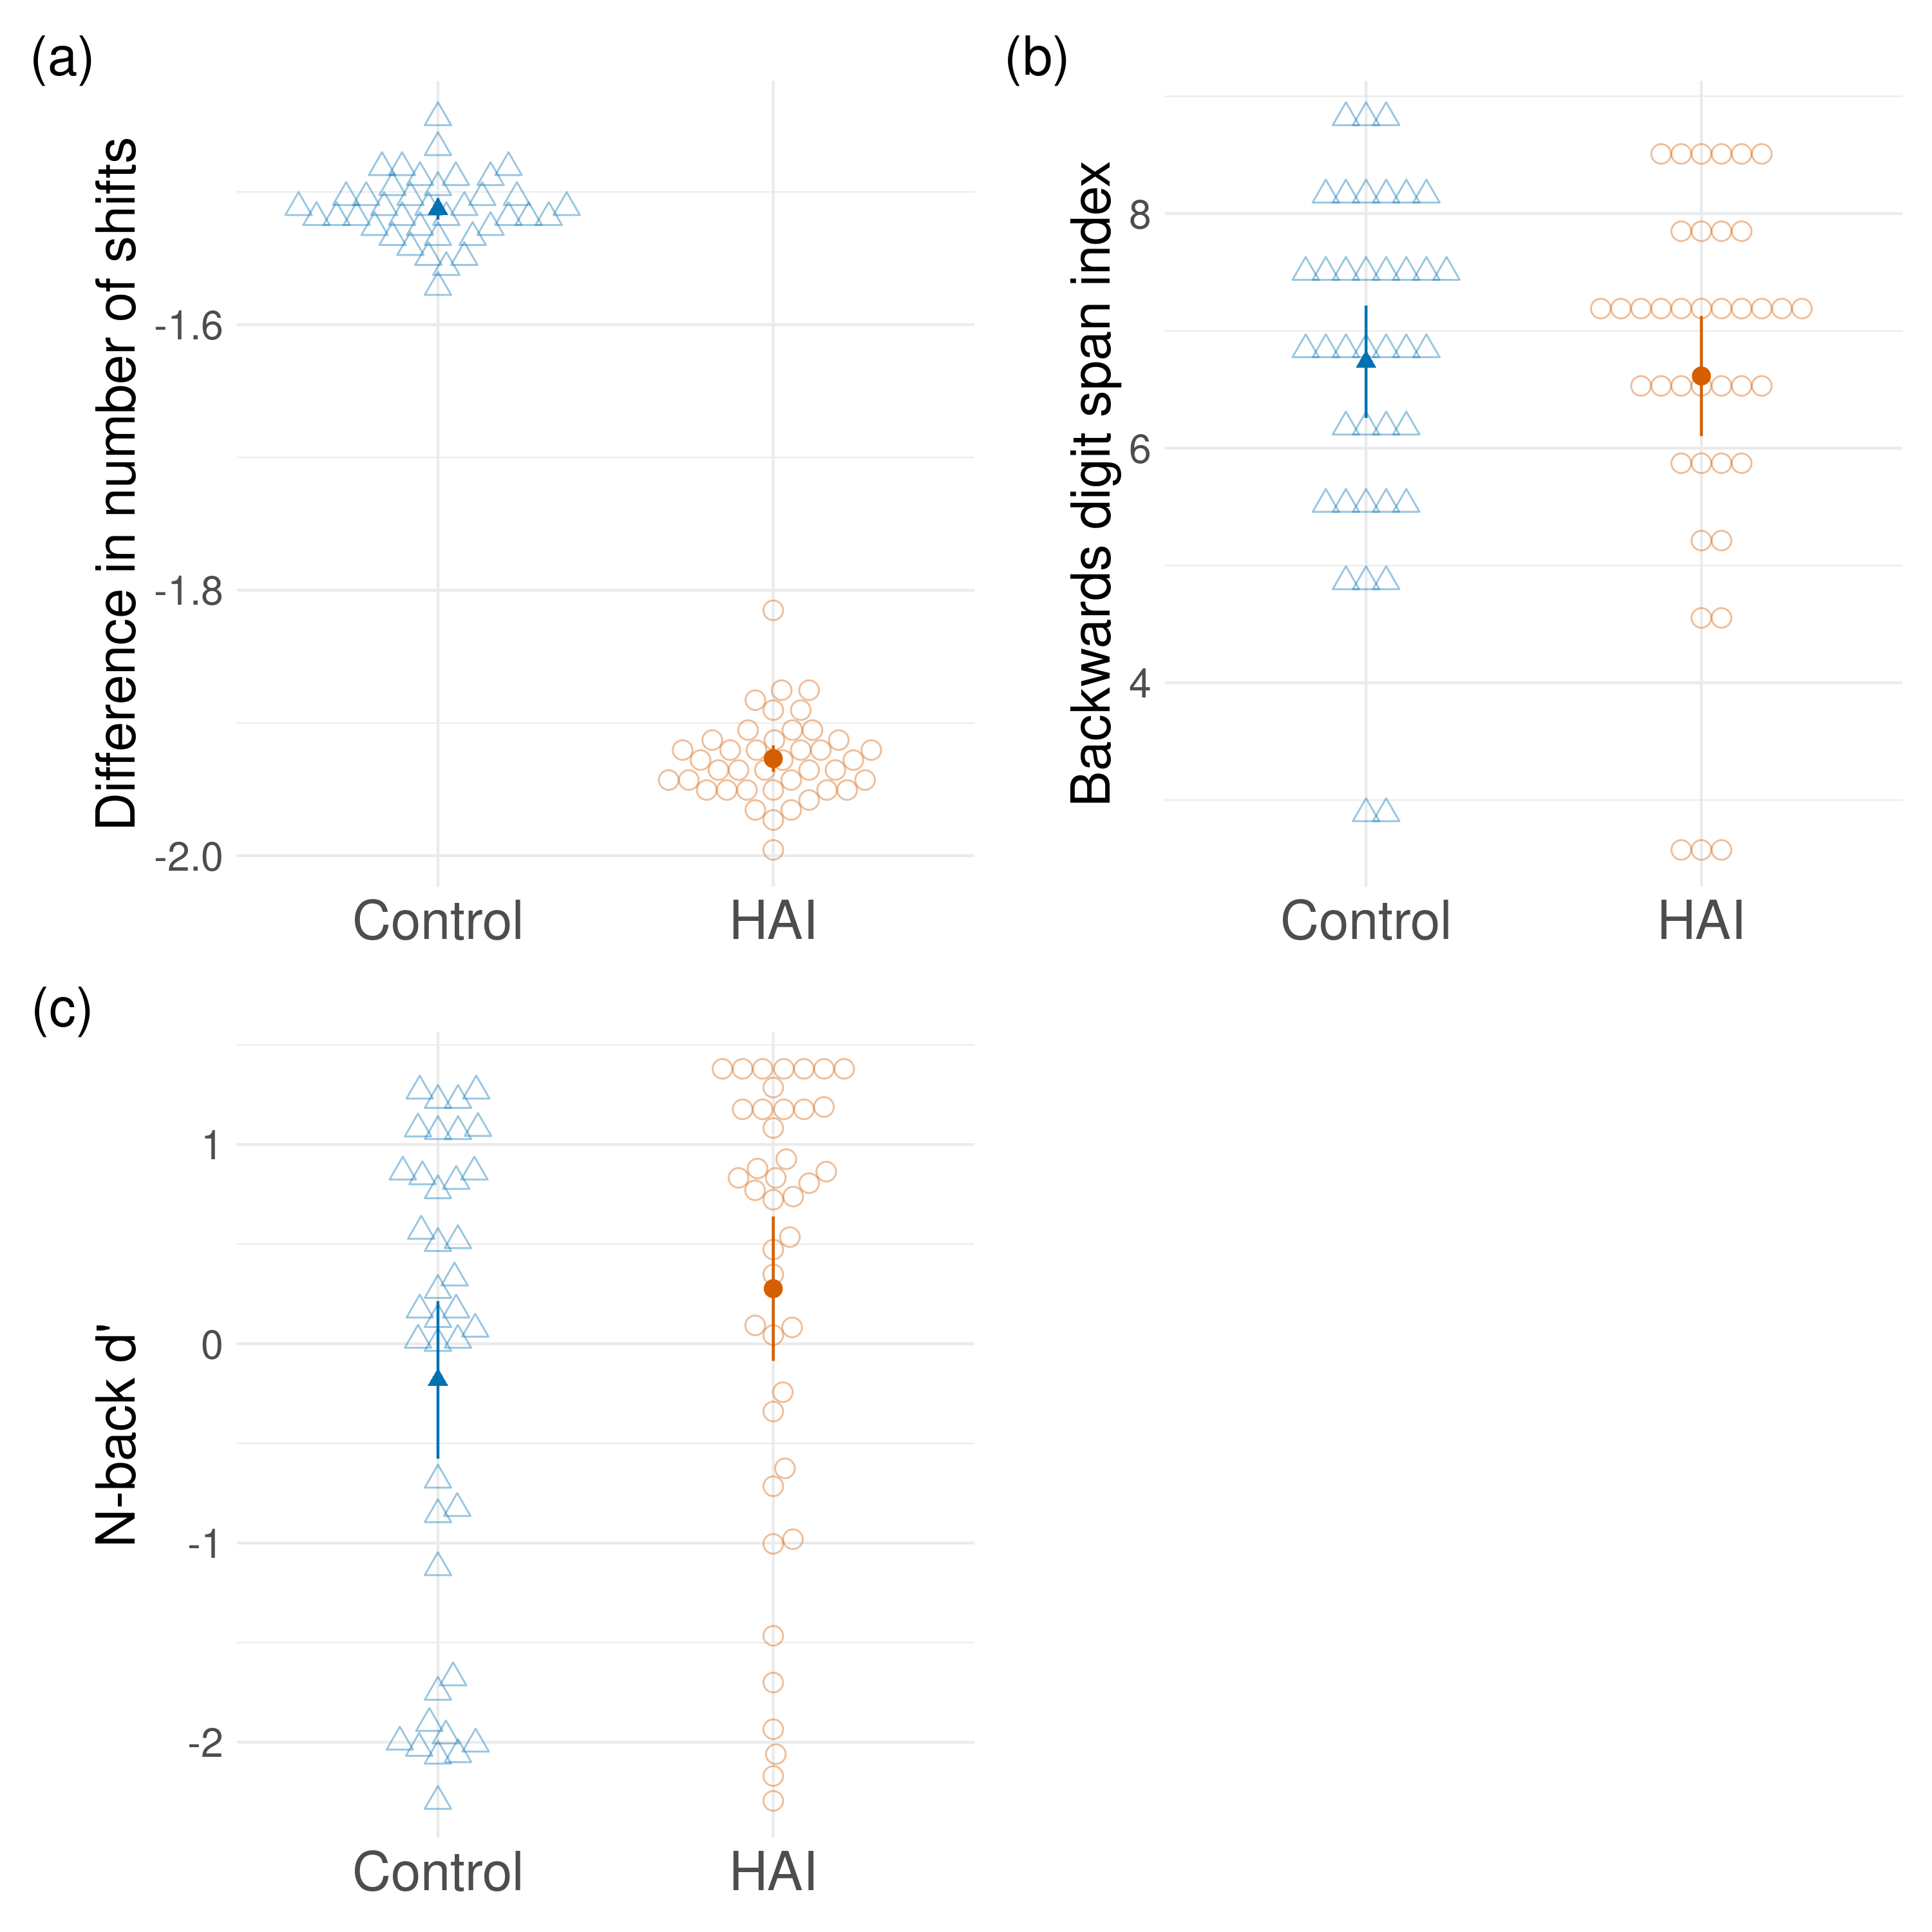
\includegraphics[width=1\linewidth]{/mnt/data/jstevens/OneDrive/active_sync/projects/haicognition2021/figures/cognitive_2} \caption{Post-condition predicted cognitive scores (controlling for pre-condition scores) for HAI (human-animal interaction) and control groups in Experiment 2. Scores show (a) the difference in number of attentional shifts between the two Necker cube trials, (b) the index for the backwards digit span task, and (c) \(d'\) for the n-back task. Open triangles (blue) represent individual control participant scores, open circles (orange) represent individual HAI participant scores, closed triangles and circles represent condition group means (with lines connecting condition means), error bars represent 95\% confidence intervals.}\label{fig:cognitive2}
\end{figure}

\clearpage


\end{document}
